\documentclass[a4paper]{paper}

\usepackage{url, graphicx, enumitem, linguex, gb4e, babel}
\usepackage[T1]{fontenc}

\renewcommand{\rmdefault}{ptm}

\begin{document}

\title{Dogs, frogs and lambs}
\subtitle{Using Constraint Grammar for Celtic languages in Apertium}
\author{ 
	{Francis M Tyers, Kevin Donnelly}
	\thanks{We are grateful to Gwenvael Jequel and ?anyone else? for help with aspects of this paper.}
	}
\date{}
\maketitle

\begin{abstract}
We describe the integration of the \textbf{vislcg3} Constraint Grammar (CG) package into Apertium, a rule-based machine translation platform.  We first give an outline of the steps necessary to achieve this integration, and then go on to consider some aspects of applying CG to the Celtic languages.
\end{abstract}

\section{Introduction}

Apertium is a machine translation platform originally developed for the Romance languages of the Iberian peninsula, but now being adapted for a variety of other languages, including Welsh \cite{Tyers2009} and Breton\footnote{ \url{http://xixona.dlsi.ua.es/~fran/breton/traductor/index.php}}.  Working systems for 17 language pairs have now been released, and all the material (both software and data) is available under the Free Software Foundation's GPL license.

The \textbf{vislcg3} constraint grammar package was integrated into Apertium in order to meet a gap in the linguistic resources available - there was no tagged corpus of Welsh available under a free license with which to train the Apertium tagger, and yet the disambiguation of the Welsh text needed to be improved before it was fed into the statistical tagger.

After a description of the integration work, we discuss the use of the CG functionality to help Apertium distinguish between homonyms in the Celtic languages.  We look at three types of homonyms: (1) those resulting from mutation, (2) interdependent homonyms, and (3) different meanings for the same part of speech.  We then discuss the use of CG to ``cast'' POS tags for homonyms (e.g. to change a subject tag for a pronoun listed in the dictionary to an object tag for a homonymous pronoun not listed in the dictionary), and go on to look at how rules from another free software package for a Celtic language (Kevin P. Scannell's \textit{An Gramad\'oir} grammar-checker for Irish) have been ported to CG.  We end with some reflections on the importance of open licensing in the development of tools for marginalised languages.

\section{Integration of \textbf{vislcg3} into Apertium}

\subsection{The Apertium pipeline}

(\textbf{Todo: Summary of the Apertium pipeline and how vislcg3 fits into it})

\subsection{Tracing the application of CG rules}

Detailed CG development depends on being able to trace which rules are being tripped during the disambiguation process. \textbf{vislcg3} already offers a mechanism for this via its \texttt{--trace} switch; the output of this is also available through Apertium.

(\textbf{Todo: Give command-line example})

Agoriad\footnote{give web address and address of git repo}, a web interface for \textbf{apertium-cy} (the Welsh version of Apertium), shows the output of each stage of the Apertium pipeline in a colour-coded tabular format.  Figure \ref{fig:ruletrace} shows CG disambiguation for:
\begin{exe}
\ex
\begin{xlist}
	\ex { \textbf{a oes lle yma?} }
	\ex { \textit{is there space here?} }
\end{xlist}
\end{exe}
To keep track of the rules, they are each named using \textbf{vislcg3}'s naming option, with some attempt being made to keep the name mnemonic.  For instance, the \textbf{R\_oes\_age} rule:\\
\indent{ \texttt{REMOVE:R\_oes\_age NC IF (-1 Vpart) (0 NC) (0 V);} }\\
will delete the noun \textbf{oes} (\textit{age}) from a \{verb, noun\} cohort if preceded by a verbal particle, to leave the desired \textbf{oes} (\textit{is}).

\begin{figure}[hbt]
	\centering
		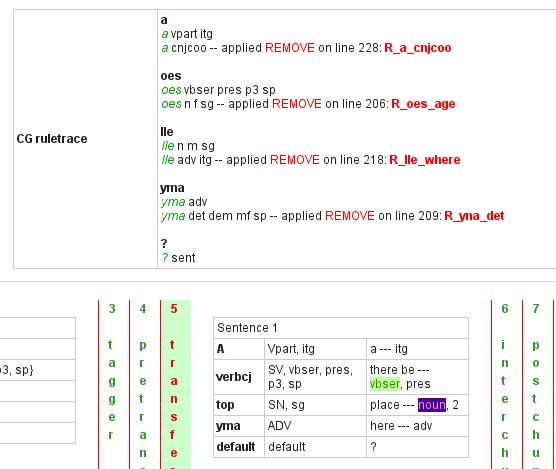
\includegraphics[width=10cm]{ruletrace.png}
	\caption{The ruletrace function of Agoriad}
	\label{fig:ruletrace}
\end{figure}

\section{Handling of mutation in Apertium}

One notable characteristic of the Celtic languages is ``mutation'' - morphophonemic alteration of initial consonants.  Consider the Welsh examples: 
\begin{exe}
\ex
\begin{xlist}
	\ex { \textbf{mae o'n marw} }
	\ex { \textit{he is dying} }
\end{xlist}
\ex
\begin{xlist}
	\ex { \textbf{mae o'n farw} }
	\ex { \textit{he is dead} }
\end{xlist}
\end{exe}
Here, the change $m \rightarrow f$ signifies that the following word is an adjective and not a verb.  In the text to be translated, these mutations have to be removed in order to get to the underlying lemma.  

In Apertium's Welsh dictionary, the entry for each mutatable word contains a reference to a paradigm which deals with the initial variants.  Thus, for \textbf{tad} (\textit{father}) we have:
\begin{quote}
\begin{verbatim}
<e lm="tad"><par n="initial-t"/><i>ad</i>
	<par n="aberth__n"/></e>
\end{verbatim}
\end{quote}

The paradigm in turn lists the various changes that can take place:
\begin{quote}
\begin{verbatim}
<pardef n="initial-t">
	<e r="LR"><p><l>t</l><r>t</r></p></e>
	<e r="LR"><p><l>d</l><r>t</r></p></e>
	<e r="LR"><p><l>nh</l><r>t</r></p></e>
	<e r="LR"><p><l>th</l><r>t</r></p></e>
	<e r="RL"><p><l>t</l><r>t</r></p></e>
</pardef>
\end{verbatim}
\end{quote}

Each line relates to a specific mutation of the base form \textbf{tad}:\\
\indent{\qquad soft mutation: \textbf{*ei tad $\rightarrow$ ei dad} - \textit{his father}}\\
\indent{\qquad nasal mutation: \textbf{*fy tad $\rightarrow$ fy nhad} - \textit{my father}}\\
\indent{\qquad aspirate mutation: \textbf{*ei tad $\rightarrow$ ei thad} - \textit{her father}}

\section{Disambiguating mutational homonyms}

This process (which is purely grapheme-based, and takes no account of the morphological significance of the mutations) allows the de-mutated lemmas to be selected, but still leaves us with a set of ambiguous choices.  CG allows the correct surface homonym to be chosen.

For instance, consider the collocation:
\begin{exe}
\ex
\begin{xlist}
	\ex { \textbf{Y Bwrdd Glo} }
	\ex { \textit{The Coal Board} }
	\ex { \textit{*The lock table} }	
\end{xlist}
\end{exe}
\textbf{Todo: The translation needs to be changed now that \textbf{glo} (coal) has been added.}\\Here, the second word, \textbf{glo}, gets returned by the dictionary as \textbf{glo} (\textit{coal}), which is correct, and also as the soft mutation (\textbf{glo}) of \textbf{clo} (\textit{lock}), which is not - a qualifier would never show a soft mutation after a masculine noun like \textbf{bwrdd} (\textit{board}).  

To deal with this, we use a CG rule as follows:
\begin{quote}
\begin{verbatim}
LIST SoftMut = ("<g.*>"ri "c.*"ri) ("<d.*>"ri "t.*"ri)
	("<f.*>"ri "b.*"ri) ("<w.*>"ri "gw.*"ri)("<b.*>"ri "p.*"ri)
	("<dd.*>"ri "d.*"ri) ("<f.*>"ri "m.*"ri);
LIST Adj = (adj);
SELECT SoftMut (-1 NF) (0 Adj);
\end{verbatim}
\end{quote}
This selects a soft-mutated adjective if it follows a noun which is feminine, but in the case above \textbf{bwrdd} is masculine, so the correct lemma, \textbf{glo} (\textit{coal}), will be selected.

Another example is a much more common one.  The surface form \textbf{chi} can be interpreted as either the second person plural pronoun (\textit{you}), by far the commonest occurrence, or as an aspirate mutation of \textbf{ci} (\textit{dog}).  In earlier versions of \textbf{apertium-cy}, we had:
\begin{exe}
\ex
\begin{xlist}
	\ex { \textbf{Gobeithio bod popeth yn iawn gyda chi.} }
	\ex { \textit{I hope everything is well with you.} }
	\ex { \textit{*Hope be everything in very with a dog.} }	
\end{xlist}
\end{exe}

The addition of the following rule:
\begin{quote}
\begin{verbatim}
REMOVE MAspC IF (NOT -1 ("ei")) (NOT -1 ("a" cnjcoo))
	(NOT -1 ("chwech"));
\end{verbatim}
\end{quote}
means that all readings with a putative aspirate mutation will be dropped if they do not follow a word listed as causing an aspirate mutation.  In more recent versions of \textbf{apertium-cy}, therefore, \textbf{chi} is properly translated:\\
\indent{ \textit{*Hope be everything in very with you.} }

\textbf{Todo: Add rule for \textbf{yn iawn} to give a better translation.}

In Breton, the verb \textbf{ober} (\textit{to do}) can be used as an auxiliary to emphasise the action of the main verb, e.g. 
\begin{exe}
\ex
\begin{xlist}
	\ex {\textbf{c'hoari a ran}} 
	\ex {\textit{I am/will be playing} (literally ``\textit{it is playing that I will do}'')}
\end{xlist}
\end{exe}
But another \textbf{ran} also exists, meaning \textit{frog}, so that early versions of \textbf{apertium-br} (the Breton version of Apertium) translated this as \textit{*play frog}.  This has been resolved with a rule to select the verb reading when it follows the relative verbal particle \textbf{a} (\textit{which}):
\begin{quote}
\begin{verbatim}
LIST VpartRef = (vpart ref);
LIST Vbloc = (vbloc);
LIST Vblex = (vblex);
LIST Vbser = (vbser);
LIST TempsFin = (pri) (pii) (past) (fti);
SET Verb = Vbloc | Vblex | Vbser;
SET VerbFin = Verb | TempsFin;
SELECT VerbFin IF (-1 VpartRef);
\end{verbatim}
\end{quote}

\textbf{Todo: Perhaps shorten this rule a bit by having less stacking.  And is the | symbol correct - should it not be +?}

\textbf{Todo: Add something about the mutation trigger rules in the Breton CG.}

\section{Disambiguating interdependent homonyms}

``Interdependent homonyms'' can be defined as a collocation in which each element is ambiguous.  But CG can often be used to resolve these ambiguities.

For example, in the Breton sentence:
\begin{exe}
\ex
\begin{xlist}
	\ex {\textbf{D'ar mare ma oan o tigeri� an nor}} 
	\ex {\textit{Au moment o� j'�tais en train d'ouvrir la porte} (\textit{While I was opening the door})}
	\ex {\textit{*Au moment mon agneau en train d'ouvrir la porte} (\textit{At the moment my lamb in process of opening the door})}
\end{xlist}
\end{exe}
both items in the collocation \textbf{ma oan} are ambiguous: \textbf{ma} can mean either \textit{my} or \textit{that}, and \textbf{oan} can mean either \textit{lamb} or \textit{[I] was}.  The combination we want (\textit{that + I was}) can be selected by using a rule:
\begin{quote}
\begin{verbatim}
LIST DetPos = (det pos);
LIST Vbloc = (vbloc);
LIST Vblex = (vblex);
LIST Vbser = (vbser);
LIST TempsFin = (pri) (pii) (past) (fti);
SET Verb = Vbloc | Vblex | Vbser;
SET VerbFin = Verb | TempsFin;
REMOVE DetPos IF (1 VerbFin);
\end{verbatim}
\end{quote}
which removes the possessive pronoun as a reading when a verb follows.

\textbf{Todo: Have I missed an additional rule to disambiguate \textbf{oan}? }

Another example from Welsh is the use of the inflected form of the preposition \textbf{i} (\textit{to}) after a temporal adverb to create the subject of a subordinate clause:
\begin{exe}
\ex
\begin{xlist}
	\ex { \textbf{cyn iddyn nhw fynd} } 
	\ex { \textit{before they go/went} }
\end{xlist}
\end{exe}
Here, \textbf{cyn} can mean either \textit{as} or \textit{before}, and \textbf{i} can mean either \textit{to} or \textit{I}.  One way of dealing with this is to have two co-dependent rules.  The first:
\begin{quote}
\begin{verbatim}
SELECT:S_cyn_cnjsub_prei ("cyn" cnjsub) (1 Prep_i);
\end{verbatim}
\end{quote}
uses the following preposition to decide that \textbf{cyn} is a subordinating conjunction \textit{before} (the other meaning of \textbf{cyn}, the co-ordinating conjunction \textit{as}, would always occur before an adjective).  Then a further rule uses the disambiguation of cyn to deal with i:
\begin{quote}
\begin{verbatim}
SELECT:S_subj_postcyn PrnSubj (-1 ("cyn"ri cnjsub));
\end{verbatim}
\end{quote}
The subject pronoun reading is selected is the subordinating conjunction \textbf{cyn} is the previous word.

\textbf{Todo: Perhaps omit the rule names here.}

\section{Disambiguating same-POS homonyms}

In each homonym group above, the individual items differed from each other in terms of their part-of-speech information.  However, Apertium can also use CG to disambiguate items in a same-POS homonym group.  For example, in Welsh \textbf{cyfeiriad} can mean \textit{address} or (less commonly) \textit{direction}.  In the sequence:
\begin{exe}
\ex
\begin{xlist}
	\ex {\textbf{i drafod cyfeiriad y bolisi} } 
	\ex {\textit{to discuss the direction of the policy} }
	\ex {\textit{*to discuss the address of the policy} }	
\end{xlist}
\end{exe}
we need to choose the less common meaning.  In the Apertium Welsh dictionary, there are separate entries for both meanings, with the less common one given the differentiating tag \textit{S1}:
\begin{quote}
\begin{verbatim}
<e><p>
<l>cyfeiriad<s n="n"/><s n="m"/></l>
<r>address<s n="n"/></r>
</p></e>

<e r="LR"><p>
<l>cyfeiriad<s n="n"/><s n="m"/><s n="S1"/></l>
<r>direction<s n="n"/></r>
</p></e>
\end{verbatim}
\end{quote}
 A CG rule can then be used to select the appropriate meaning by substituting the \textit{S1}-tagged entry for \textbf{cyfeiriad} when the verb \textbf{trafod} precedes it:
\begin{quote}
\begin{verbatim}
SUBSTITUTE ("cyfeiriad"ri n m) ("cyfeiriad" n m S1) NC 
(-1 ("trafod"ri vblex));
\end{verbatim}
\end{quote}

\section{Casting of POS tags}

Moving on from the disambiguation of same-POS homonyms, we are exploring the implications of using CG to do pre-processing of polysemous lemmas (i.e. homonyms with related meanings) by adjusting their tags based on surrounding text.  For instance, compare the two sentences:
\begin{exe}
\ex
\begin{xlist}
	\ex {\textbf{Mi welsom ni y bachgen a'n ffrindiau ar y traeth.} } 
	\ex {\textit{We saw the boy and our friends on the beach} }
\end{xlist}
\end{exe}
\begin{exe}
\ex
\begin{xlist}
	\ex {\textbf{Mi welodd y bachgen ni a'n ffrindiau ar y traeth.} } 
	\ex {\textit{The boy saw us and our friends on the beach} }
	\ex {\textit{*The boy saw we and our friends on the beach} }	
\end{xlist}
\end{exe}
The lemma \textbf{ni} is polysemous between \textit{we} (subject) and \textit{us} (object).  The entry in the Apertium Welsh dictionary is for the subject meaning only, so the second sentence will have the sub-optimal translation \textit{we} instead of the desired \textit{us}.  It would be possible to add another dictionary entry for the object meaning, and use a CG rule to select it whenever \textbf{ni} is not preceded by a first-person plural verb, but a shortcut to the same result is to cast the subject tag attached to \textbf{ni} to an object tag, using a rule such as:
\begin{quote}
\begin{verbatim}
SUBSTITUTE (subj) (obj) prn_subj_1pl (NOT -1 vb_1pl);
\end{verbatim}
\end{quote}

Another alternative for dealing with this would be to remove the subject tag from the dictionary entry for \textbf{ni}, and then MAP a syntax tag onto it as required:
\begin{quote}
\texttt{Rwyf/Bod<vbser><pres><p1><sg>}\\
\texttt{i/prpers<prn><p1><mf><sg><@$\leftarrow$SUBJ>}
\end{quote}
This would involve changes to the bilingual dictionary and the transfer rules.  The idea would be to map to subject tags first, and then use CG rules to map to object where necessary.

\textbf{Todo: Can you say more about this?  Should we weigh up pros and cons, or is it a bit pointless?}

\section{Porting of An Gramad\'oir rules for Irish}

CG has already been used for Irish \cite{uiDhonnchadha2006}, with over 300 rules being reported.  Given the relative lack of resources for marginalised languages, we were anxious to re-use work already done by Kevin Scannell on his Irish grammar-checker, and the first author has ported the disambiguation rules there to the \textbf{vislcg3} format.  

\textbf{Todo: Say more about why, how, and benefits.}

\section{Discussion}

Although the integration of \textbf{vislcg3} into Apertium began as an ad hoc means of adding functionality, it has now become a much more important part of the Apertium pipeline.  Currently, there are \textbf{xx}, \textbf{yy} and \textbf{zz} CG rules for Welsh, Breton and Irish respectively, and it is likely that the scope of the rules will expand as we become more adept at using them creatively.

It is worth noting that without the GPL licensing of \textbf{vislcg3} it would not have been possible to use it in Apertium.  This would have meant coding something similar for Apertium, instead of spending that time improving the translation fidelity.  In turn, this would have meant that the insights derived from applying CG to a couple of new languages would have been lost.  GPL licensing, where both the software and the data are available for interested researchers to examine, has ensured optimal results for blah blah

\textbf{Todo: This is crap - perhaps you can do better, or I'll look at it again tomorrow.}


\begin{thebibliography}{9}
                                                                
\bibitem{Tyers2009} \textsc{Francis M. Tyers and Kevin Donnelly}:\ \textit{apertium-cy -- a collaboratively-developed free RBMT system for Welsh to English}, Prague Bulletin of Mathematical Linguistics, 91, (2009), 57-66.

\bibitem{uiDhonnchadha2006} \textsc{Elaine U\'i Dhonnchadha and J. Van Genabith}:\ \textit{A Part-of-speech tagger for Irish using Finite-State Morphology and Constraint Grammar Disambiguation}. 

\end{thebibliography}

\textbf{Todo: Need to add more references, eg Scannell, GPL papers.  Some details are missing for U\'i Dhonnchadha, and perhaps we should use a separate bibliography file.}


\end{document}

